\chapter{Visualizers}

To show the capabilities or our designed \emph{framework} and \emph{platform}, we decided to implement two concrete visualizers: D3.js Chord Visualizer and Google Maps Visualizer.

\section{D3.js Chord Visualizer}
\label{sec:visualizers:chord}

The D3.js Chord Visualizer is a brand new \emph{visualizer} that has not existed before in LinkedPipes Visualization. The core of this \emph{visualizer} is a chord diagram which is a method of visualizing the relationships among a group of entities (the data are usually represent using a square matrix). The diagram is in a form of a circle around which the entities are drown. The relationships between the entities are represent using arcs connecting them.

\begin{figure}
	\centering
	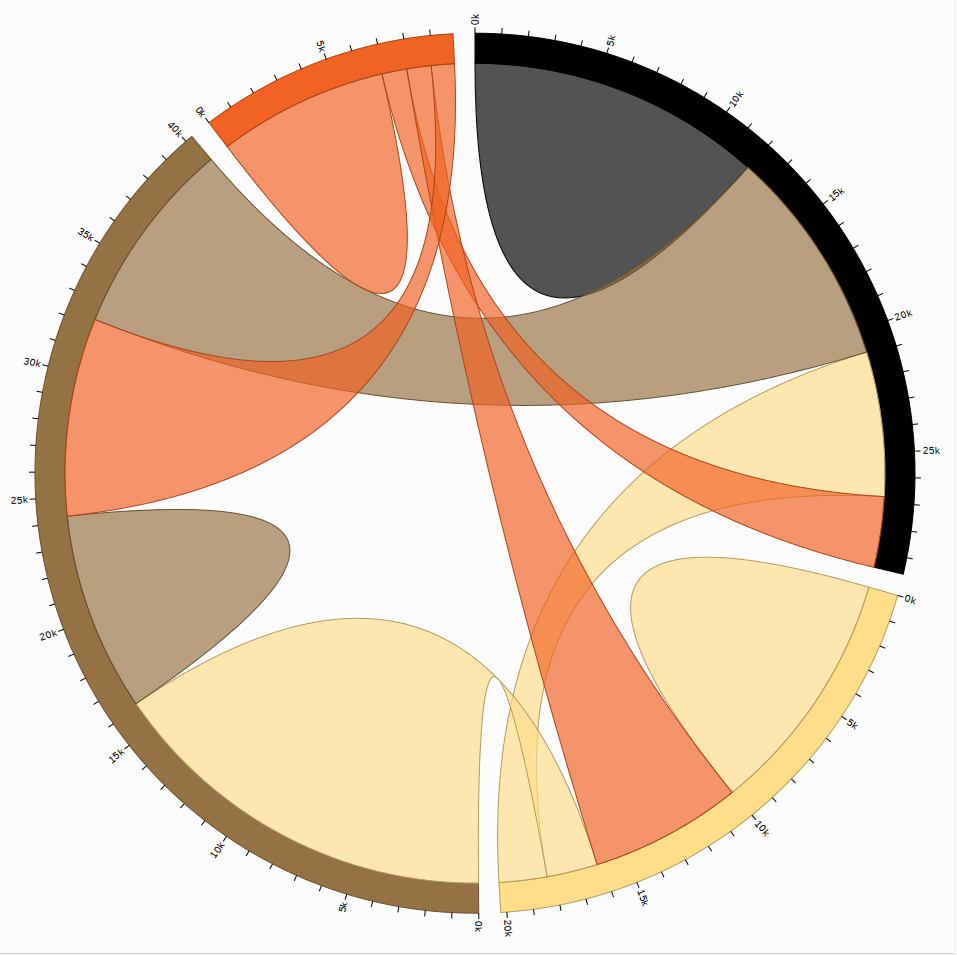
\includegraphics[width=110mm]{img/06_chord_example.png}
	\caption[Sample chord visualization]{Sample chord visualization (image source\footnotemark)  }
	\label{fig:chord-example}
\end{figure}

\footnotetext{http://bl.ocks.org/mbostock/4062006}

\subsection{Sample data sets}
\label{sec:visualizers:chord:data-sets}

We used three different data sets to demonstrate the abilities of this \emph{visualizer}.

\begin{enumerate}

\item \textbf{Registry of contracts of Czech Republic}
% [cite: http://internal.opendata.cz/dataset/gov-cz-smlouvy]

Database of contracts between private businesses and public government organizations (ministries, towns etc). The chord diagram could be used to visualize economic activity between individual business entities.

\item \textbf{UNHCR Population Statistics – Asylum seekers by months} 
% [cite: http://popstats.unhcr.org/en/asylum_seekers_monthly]

This database contains information about people from all over the world asking for asylum outside of their home countries. The database contains concrete numbers of people coming from one country to another, divided by months. The chord visualizer would be able to nicely visualize the trends of people moving around the globe.
% * <tobiaspotocek@gmail.com> 2016-06-27T15:29:26.094Z:
%
% > globe
%
% Jirka Helmich: kde jste ho vzal, jak jste ho vyrobil, citace ETL http://2016.eswc-conferences.org/sites/default/files/papers/Accepted%20Posters%20and%20Demos/ESWC2016_DEMO_Linked_Pipes_ETL.pdf
%
% ^ <tobiaspotocek@gmail.com> 2016-06-27T15:29:46.740Z:
%
% Toto zmiňuji o něco dále. Jakým způsobem jsou data sety převedeny do RDF a do RGML vocabulary. Musím to nějakým způsobem zmínit už zde?
%
% ^.

\item \textbf{OpenFlights – Air routes} 
% [cite: http://openflights.org/]

Database of airports and air routes between them from all over the world. Although air routes are not as informative as actual passenger numbers between individual destinations (that information is to our best knowledge not available), they still give a pretty good idea about overall traffic and people movements. Using a chord diagram, we can visualize traffic intensity between individual airports. This data set is also by far the largest one, consisting of around 8000 airports and almost 70000 air routes.

\end{enumerate}
These data sets are very different but they all contain information about some kind of relations which can be (with various results) visualized using a chord diagram. 

\subsection{LDVM visualizer component}

As this \emph{visualizer} was completely new, we had to start by defining the LDVM \emph{visualizer component}.

The core aspect is defining the component \emph{descriptor}, i. e., what the data should look like so that our \emph{visualizer} can visualize it. Obviously, our goal was to design a universal visualizer that could work with any data containing relationships, not just the three mentioned data sets. Therefore we focused on describing the universal shared nature of the data.

In the very beginning, we were considering the option of creating a brand new RDF vocabulary. The chord visualization was pretty uncommon in the world of Linked Data, so it would be justifiable to come up with a specialized vocabulary. Nevertheless, after some further analysis we came to realization that what the chord diagram actually visualizes is a weighted (optionally directed) multi-graph (as understood in the graph theory).

Let us look at our data sets again:

\begin{itemize}
\item The main entity in the Registry of contracts is (not surprisingly) a contract. A contract has two parties. The transition to graph vocabulary is very clear here. A contract is an edge, each party is a vertex. In this case, the graph is undirected as the partners are equal. There can be multiple contracts between two parties, so it is a multi graph. As we are not interested in the individual contracts, but rather in the number of them, all contracts between two parties could be aggregated into a single weighted undirected edge.
\item The asylum seekers data set consists of individual records where each record contains a period of time, country of origin, country of asylum and a number of people stating how many people sought asylum during that period of time between those two countries in this specified direction. Clearly, each record corresponds to an edge and each country corresponds to a vertex. The weight of an edge represents number of people. Unlike in the previous example, this time the graph is directed as it actually matters which direction the people went. Therefore a relationship between two vertices is asymmetrical. That can also be visualized using the chord diagram.
\item The air routes data set is a combination of the previous two cases. Each air route corresponds to an edge which is directed but is not by default weighted. To express the strength of a relationship, all edges of the same direction between two airports should be merged into one weighted edge.
\end{itemize}

% [cite: http://www.cs.rpi.edu/research/groups/pb/punin/public_html/RGML/EXTREME/rgml_ext.html]
Now that we had described the actual universal nature of the data visualizable by the chord diagram (a graph), it became much clearer what kind of vocabulary we would need. We were pretty certain that we would hardly be the first with the need to describe a graph in RDF. Unsurprisingly, it did not take us long to come across the RGML vocabulary which was designed with this exact purpose in mind.

\subsection{Describing graphs using RGML vocabulary}
\label{sec:visualizers:chord:rgml}

Let us briefly describe the vocabulary. It contains these three most important classes: \texttt{rgml:Graph}, \texttt{rgml:Node} and \texttt{rgml:Edge}. The purpose of those classes is self-explanatory, nevertheless, we would like to make two remarks. Firstly, until now we have been using the term \emph{vertex} which is probably more common in graph theory. To maintain consistency with the RGML vocabulary, from now on, we will strictly stick to the term \emph{node}. Secondly, whenever we will use the term graph, we will be speaking about an actual graph structure described using the RGML vocabulary, not the RDF named graph.

The vocabulary also defines several different properties but we will describe only those most important ones. Each edge can define its source node and target node using properties \texttt{rgml:source} and \texttt{rgml:target}. Clearly, an edge is intrinsically directed. The question is whether it should be also always understood as directed. That is defined by a graph boolean property \texttt{rgml:directed}. The vocabulary allows to use this property also directly on edges which makes it possible to create mixed graphs, i. e., graphs containing both directed and undirected graphs. We did not find this feature useful for our purposes so we do not support it. There is also the \texttt{rgml:label} property which we decided to ignore and use  \texttt{rdfs:label} instead. One of the reasons was that the \emph{framework} (see Subsection \ref{sec:implementation:advanced-features:label-dereferencering}) would not be able to automatically fetch missing labels defined with the \texttt{rgml:label} property.

Let us now have a look at a concrete example. This is a data sample from the registry of contracts data set:

\begin{verbatim}
PREFIX gr: <http://purl.org/goodrelations/v1#>
PREFIX rejstriky: <http://linked.opendata.cz/ontology/domain/seznam.gov.cz/rejstriky/>
PREFIX profiles: <http://linked.opendata.cz/ontology/buyer-profiles/>
PREFIX smlouvy: <http://linked.opendata.cz/resource/domain/seznam.gov.cz/smlouvy/>
PREFIX businessentity: 
    <http://linked.opendata.cz/resource/domain/seznam.gov.cz/rejstriky/business-entity/>

<http://linked.opendata.cz/resource/business-entity/CZ00283924> a gr:BusinessEntity ;
    rejstriky:smlouva smlouvy:260167803 
    .
        
smlouvy:260167803 a rejstriky:Smlouva ;
    rejstriky:partner businessentity:67028144 
    .
\end{verbatim}

The second resource of type \texttt{rejstriky:Smlouva} is a contract between the first entity (the one of type \texttt{gr:BusinessEntity}) and the entity marked as \texttt{rejstriky:partner} of the contract. Augmented with the RGML vocabulary, the data would look like this:

\begin{verbatim}
PREFIX rgml: <http://purl.org/puninj/2001/05/rgml-schema#> .
PREFIX smlouvy: <http://linked.opendata.cz/resource/domain/seznam.gov.cz/smlouvy/>
PREFIX businessentity: 
    <http://linked.opendata.cz/resource/domain/seznam.gov.cz/rejstriky/business-entity/>

smlouvy:260167803 rdf:type rgml:Edge ;
    rgml:source <http://linked.opendata.cz/resource/business-entity/CZ00283924> ;
    rgml:target rejstriky:partner businessentity:67028144 ;
    rgml:weight "1" 
    .
    
<http://linked.opendata.cz/resource/business-entity/CZ00283924> rdf:type rgml:Node .
businessentity:67028144 rdf:type rgml:Node . 
\end{verbatim}

We used the word \emph{augmented} on purpose because we believe that it perfectly describes what happened here. We did not add any information that was not already there. We just used a different vocabulary to express the same information. A vocabulary that our visualizer understands.

Nevertheless, it is clear that some kind of data transformation has to be performed. For this particular data set we created a reusable LDVM \emph{analyzer component} that is responsible for this augmentation. That means that it can take any data in the suggested format and enhance it with the RGML vocabulary to make it understandable by the chord \emph{visualizer}.
	
% [cite - http://etl.linkedpipes.com/]    
A similar approach was applied for the other two data sets as well. Unlike the contracts, these data sets were not already in RDF, they were simple CSV files. We converted them to RDF with an external (but related) tool, LinkedPipes ETL. As we were responsible for the conversion, we used directly the RGML vocabulary for the output, as there was no point in creating an intermediate step.

When we were describing the individual data sets, we mentioned several times the need (or possibility) to perform an aggregation on the data (for example, merging all contracts into one weighted undirected edge). We decided to leave this part to the \emph{visualizer}. Because of the way the chord diagram works, it does not matter whether the underlying graph contains 10 edges of weight 1 between two nodes, or a single edge of weight 10. Therefore the \emph{visualizer} will behave the same and if necessary, it will perform the aggregation itself. It is important to note that this aggregation will be performed on the server-side, i.e., it will not be required to transfer the whole data set to the client first. 

Besides the mentioned augmentation, it is necessary to provide one piece of extra information for the \emph{visualizer}, and that is whether the graph is directed or undirected. We do that by creating an instance of \texttt{rgml:Graph} which will contain that information.

\begin{verbatim}
PREFIX rgml: <http://purl.org/puninj/2001/05/rgml-schema#> .
PREFIX : <http://linked.opendata.cz/ontology/temporary/chord#>

:graph rdf:type rgml:Graph ;
    rgml:directed false
    .
\end{verbatim}

%[cite - "specification" -> RGML]
%[cite - https://www.w3.org/TR/rdf-schema/ rdfs]
%[cite - https://www.w3.org/TR/sparql11-property-paths/ sparql11-propert-paths]

Here we feel it is important to mention one limitation of this \emph{visualizer}. The RGML vocabulary requires the individual nodes and edges to be tied to a concrete instance of \texttt{rgml:Graph} using predicates \texttt{rgml:nodes} and \texttt{rgml:edges}. The problematic aspect here is that, according to the specification [cite rgml], both of these predicates expect RDF Bag as the value.

RDF Bag \cite{rdf_vocab} is a container whose structure resembles linked list and it is pretty inconvenient to work with using standard SPARQL queries. As of selecting all graph nodes using a single \texttt{SELECT} query, RDF Schema defines a special property \texttt{rdfs:member} which should make it possible. However, this property has to be explicitly supported by the SPARQL engine 
\footnote{\url{https://lists.w3.org/Archives/Public/public-rdf-dawg-comments/2007Jun/0005.html}} which is not always the case 
\footnote{\url{http://stackoverflow.com/a/16130842/576997}}, definitely not for Virtuoso
\footnote{\url{http://stackoverflow.com/questions/27124941/how-to-run-rdfsmember-on-a-sparql-endpoint}}
\footnote{\url{http://stackoverflow.com/questions/27046770/add-rdfs-inference-rules-support-in-endpoint-sparql}} (our experiments showed that as well). Some engines offer their own proprietary solutions 
\footnote{\url{http://answers.semanticweb.com/questions/18056/querying-rdf-lists-collections-with-sparql}} to address this issue but that was something we wanted to avoid. Eventually, we had more luck with \emph{property paths} defined by the SPARQL 1.1 standard [cite sparql11-property-paths] which actually do allow selecting Bag content with a single query.  As of constructing a Bag of nodes using  a \texttt{CONSTRUCT} query, it does not seem to be possible at all 
\footnote{\url{https://www.w3.org/2009/sparql/wiki/Feature:Constructing\_containers\_and\_collections}}. This is something that an \emph{analyser} augmenting the data with RGML vocabulary would typically need. The point of this paragraph was to show that the support of this RDF container is not ideal and that we would rather avoid using it.

We decided to make a compromise. We simply always expect that all existing edges and nodes belong to the same graph. In other words, this \emph{visualizer} does not officially support multiple graphs within the same data set. Practically, it does to a certain extent. The nodes of different graphs will not be connected in any way, so basically our \emph{visualizer} will consider them separated connected components within a single graph. As the user will be allowed to specify the graph nodes that he wants to visualize, this will not have any practical impact on the visualization (he will manually select the subgraph he is interested in). The only situation when this would cause undesired behavior would be the case when some graphs would be directed and some graphs undirected. 

So even though this limitation exists, we do not consider it limiting for the user. Typically, the \emph{visualizer} will be working with a data set produced by a \emph{pipeline} which means the \emph{visualizer} will be operating within a single named RDF graph and in this situation any conflicts are unlikely. Of course, if the user selects a data source with a large number of different graphs (for example by choosing a whole SPARQL endpoint without specifying the named graph), it might be difficult for him to make any meaningful visualizations.

The initial question in this part was how would the \emph{descriptor} of a LDVM \emph{visualizer component} look like. Based on the thought process described in the previous paragraphs, we ended up with the following result:

\begin{verbatim}
PREFIX rdf: <http://www.w3.org/1999/02/22-rdf-syntax-ns#>
PREFIX rgml: <http://purl.org/puninj/2001/05/rgml-schema#>

ASK {
    ?graph rdf:type rgml:Graph ;
        rgml:directed ?directed 
        .
            
    ?edge rdf:type rgml:Edge ;
        rgml:source ?source ;
        rgml:target ?target ;
        rgml:weight ?weight 
        .
            
    ?source rdf:type rgml:Node .
    
    ?target rdf:type rgml:Node .
}
\end{verbatim}

To be more precise according to \cite{ldvm_use_cases}, this is the \emph{descriptor} of the only \emph{mandatory feature} of LDVM chord \emph{visualizer component}.

\subsection{Making the graph searchable with FRESNEL vocabulary}

% TODO: add a figure with too many nodes

Until now we have been discussing how to describe the data themselves and how to make them visualizable with the chord diagram. Now let us move to another challenge. The chord diagram can effectively visualize only a limited number of nodes. According to our experiments, this number is somewhere around 30. That does not mean that the diagram is not able to visualize more, it just means that it might be hard for the user to make out any sense out of such diagram (see Figure). Plus there might be related performance issues. Unfortunately, the graphs we are working with have hundreds or even thousand of nodes. Clearly, we need to come up with a way to allow the user to explore the graph and define what should be visualized.

Our first obvious choice we considered was some kind of filtering. But we quickly realized that it was not really applicable to our testing data sets as they do not provide any information (like a hierarchical structure) that we could use. We needed something more universal.

The contracts were the first data set that we experimented with. Each contract is between two parties which are organizations or business entities, usually identified with their name or their VAT number. We tried to imagine how a user would interact with such data and we came to the conclusion that one of the possible use cases would be that the user already knows what he is looking for (in this case, a name of a contractor, or its VAT number) and wants to visualize this particular company and its partners. So the approach would be to let the user simply search through the graph for the nodes he is interested in. That brings up many further questions, at this moment mainly how to define what data (more specifically, which node properties) should be searchable.

The input data are in RDF which means that each node can have an arbitrary (and possibly very large) number of properties. Obviously, we could use a fixed set of searchable properties (for example \texttt{rdfs:label} would be one candidate) but that would not be very flexible if we wanted to support data from different domains in the future. Instead, we decided to let the data set itself define the searchable properties. The only thing missing was a vocabulary that would allow us to express such facts.

% [cite: https://www.w3.org/2004/09/fresnel FRESNEL]
We went through similar thought process as in the previous part, considering our own proprietary vocabulary, but eventually we ended up with FRESNEL. This vocabulary is fairly complicated, so we will just explain the main ideas. It makes it possible to extend existing RDF data with presentational metadata. More specifically, it allows to define what information should be presented and how it should be presented. This does not exactly sound like what we need here but what is important, it allows us to do what we need.

One of the two main FRESNEL concepts are \emph{lenses}. A \emph{lens} is representing a “view” on data (it is very similar to a projection from database theory). A \emph{lens} defines a type of resource and a list of its properties that should be presented when using this \emph{lens}. In our case, we do not present those properties, we search them.

Here is an example of a \emph{lens} which specifies searchable properties in the contracts data set:

\begin{verbatim}
PREFIX fresnel:  <http://www.w3.org/2004/09/fresnel#>
PREFIX : <http://linked.opendata.cz/ontology/temporary/chord#>
PREFIX gr: <http://purl.org/goodrelations/v1#>
PREFIX profiles: <http://linked.opendata.cz/ontology/buyer-profiles/>

:searchableLens rdf:type fresnel:Lens ;
    fresnel:purpose "searchable" ;
    fresnel:classLensDomain rgml:Node ;
    fresnel:showProperties ( gr:legalName profiles:dic ) 
    .
    
profiles:dic
    rdfs:label "DIČ"@cs ;
    rdfs:label "DIC"@en 
    .
    
gr:legalName
    rdfs:label "Název subjektu"@cs ;
    rdfs:label "Legal name"@en 
    .
\end{verbatim}

Notice two things. Firstly, using the \texttt{fresnel:purpose} property we specify what the \emph{lens} should be used for (the \emph{visualizer} will be looking for a \emph{lens} with the \emph{searchable} purpose). Secondly, what we do here is that we add labels for the searchable properties. The labels are used later when creating the user interface.

From now on, we will refer to this \emph{lens} as to the \emph{searchable lens}.

We believe that this is one of the moments that clearly show that our \emph{application generator} is truly data-driven as even the user interface dynamically adapts to the data itself. We do admit that this statement depends on one’s perspective. The \emph{searchable} lens could be considered a part of the application configuration. But from a bigger perspective, this is nothing else than just some extra metadata that are part of the data set. They can be used by any \emph{visualizer}, not just this one, and the actual application configuration begins in later phases. Note that we already came across this dilemma when we were describing the Miga Data Viewer (see Section \ref{sec:related-work:miga-data-viewer}).

Here we should mention couple of limitations that this approach has. Mainly, all the searchable properties must be literals. For example, if a node has an address which is not a literal but a structured RDF resource of type \texttt{schema:PostalAddress}, then the individual fields (street, city, country) cannot be searched. Moreover, there are couple of drawbacks stemming from the actual implementation, but that will be mentioned later.

One last thing in this part. We need to accordingly extend the LDVM \emph{visualizer component}. This becomes another \emph{feature} of the component but unlike the graph data, this one is not \emph{mandatory}. Without the graph data, the \emph{visualizer canno}t work, there is nothing to visualize. Without the \emph{searchable lens}, the usability of the \emph{visualizer} will be limited (it just displays a random sample visualization of the graph) but the core functionality will not be breached. So we extend the component with an \emph{optional feature} with the following \emph{descriptor}:

\begin{verbatim}
PREFIX rdf: <http://www.w3.org/1999/02/22-rdf-syntax-ns#>
PREFIX rgml: <http://purl.org/puninj/2001/05/rgml-schema#>
PREFIX fresnel:  <http://www.w3.org/2004/09/fresnel#>
ASK {
    ?searchableLens rdf:type fresnel:Lens ;
        fresnel:purpose "searchable" ;
        fresnel:classLensDomain rgml:Node ;
        fresnel:showProperties ?properties
        .
}
\end{verbatim}

\subsection{Configurator user interface}

Until now we have been discussing the data. Their format, nature, description. Let us now move to the actual application user interface which is built on top of the data. 

% TODO: ref to the figure with too many nodes

As we already mentioned, the chord diagram is only capable of visualizing around 30 nodes. Obviously, it can visualize more, but 30 is an upper bound for when the user is still able to make some sense out of the visualization. To deal with this limitation, we decided to introduce a concept of \emph{named lists}. While in the \emph{configurator}, the user can create a list, give it a name and add nodes to it (Figure \ref{fig:chord-named-list}). When he is happy with the result, he hits the \textbf{Visualize} button, and a chord diagram showing relationships between selected nodes is generated. The diagram is interactive. When user hovers over nodes or chords (edges), adjacent entities are highlighted and a label with some extra information is shown. The user can create multiple \emph{named lists}. Each list basically represents a different visualization and all visualizations can exist together within a single application.
\begin{figure}
	\centering
	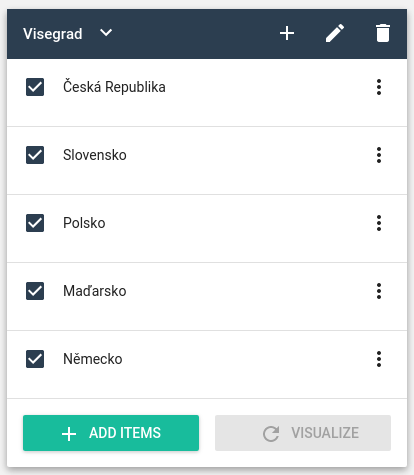
\includegraphics[width=50mm]{img/06_chord_named_list.png}
	\caption{D3.js Chord Visualizer: Named list}
    \label{fig:chord-named-list}
\end{figure}

The process of adding nodes to a \emph{named list} is leveraging the FRESNEL \emph{searchable lense}. When the user desires to add more nodes to the  list, he opens a dialog using which he can search the graph nodes. Let us say that the user is working with the air routes data set and is interested in British airports. All he has to do is open the dialog and search for “United Kingdom” (Figure \ref{fig:chord-search-dialog}). This works because each airport has a country attached to it and this particular property is marked as searchable with the FRESNEL vocabulary.

This rather elegant way allows the user to work with the graph data. Adding the nodes one by one is nevertheless still a little cumbersome. To improve usability, we implemented a functionality which enables the user to select not just one node from the search result, but also all its related nodes (in graph theory we would say all adjacent nodes). This proves itself to be very useful as it addresses pretty common scenarios. Let us say we are interested in all air routes coming to Prague. Or we want all asylum seekers coming to Czech Republic. Or we want all business partners of a certain company. This functionality allows us to get results for all these cases. On top of that, the \emph{configurator} respects properties of the graph, i. e., if the graph is directed, the user can specify which nodes interest him, whether those connected by outgoing edges or incoming edges.

\begin{figure}
	\centering
	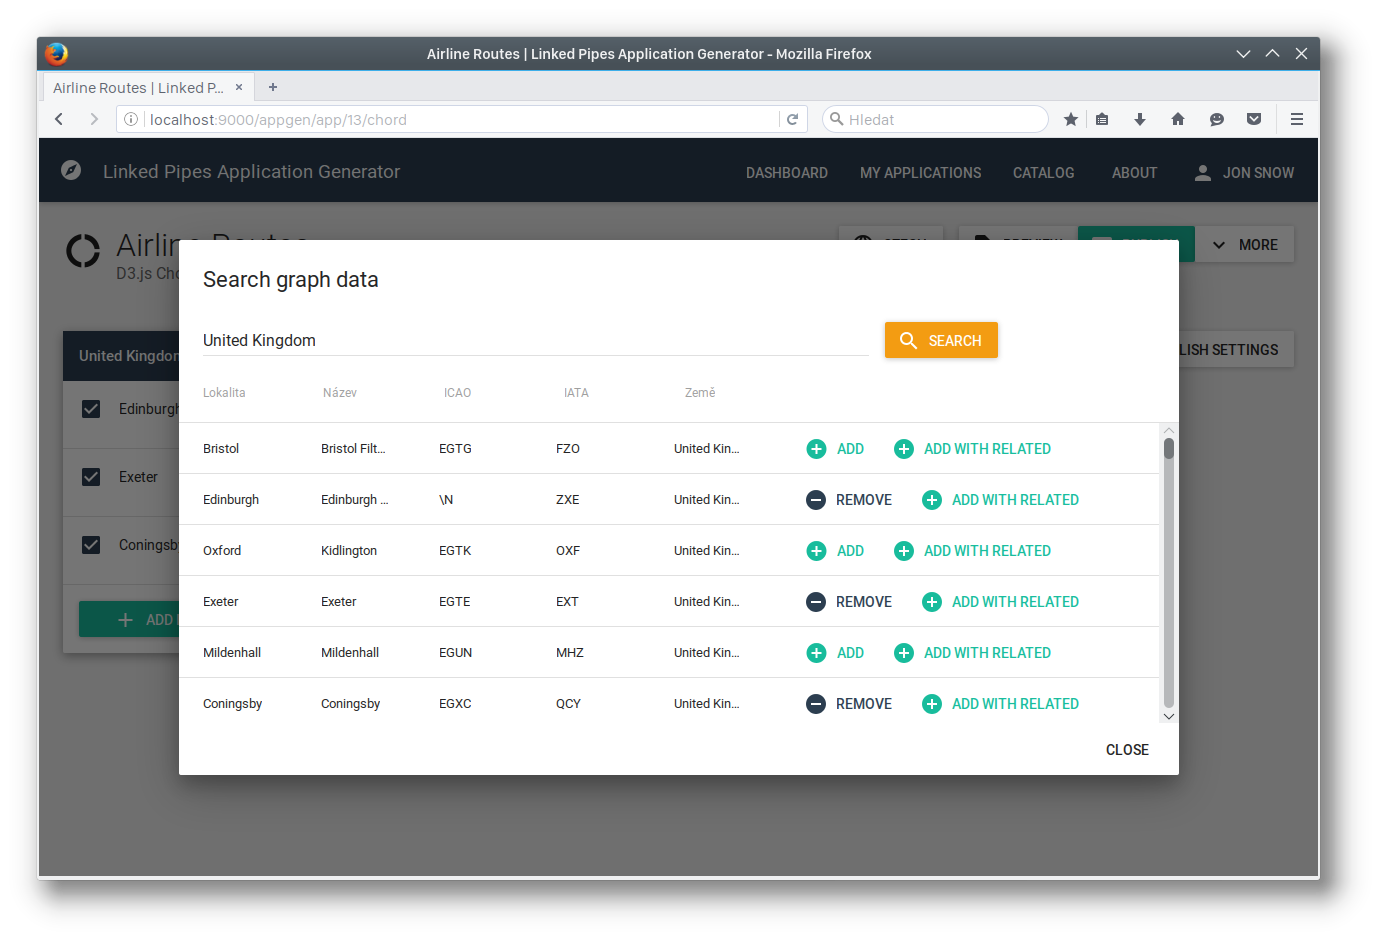
\includegraphics[width=145mm]{img/06_chord_search_dialog}
	\caption{D3.js Chord Visualizer: Search dialog}
    \label{fig:chord-search-dialog}
\end{figure}

It is important to say here that all of this works only when the \emph{searchable lens} is available. Without the \emph{searchable lens} the \emph{visualizer} is not able to reason in any way about the graph and does not offer any way to browse the nodes (the number of nodes can be very large). In this case it simply displays a random sample of the graph.

Now is the time to talk about one crucial limitation of this way of visualizing relationships. In the previous paragraphs we mentioned an example of what we might be interested in: all asylum seekers coming to Czech Republic. Let us start there. We create a new list, search for Czech Republic and add all countries from which there are incoming asylum applications. The Figure \ref{fig:chord-immigration-to-cr-1} shows the results.

\begin{figure}
	\centering
	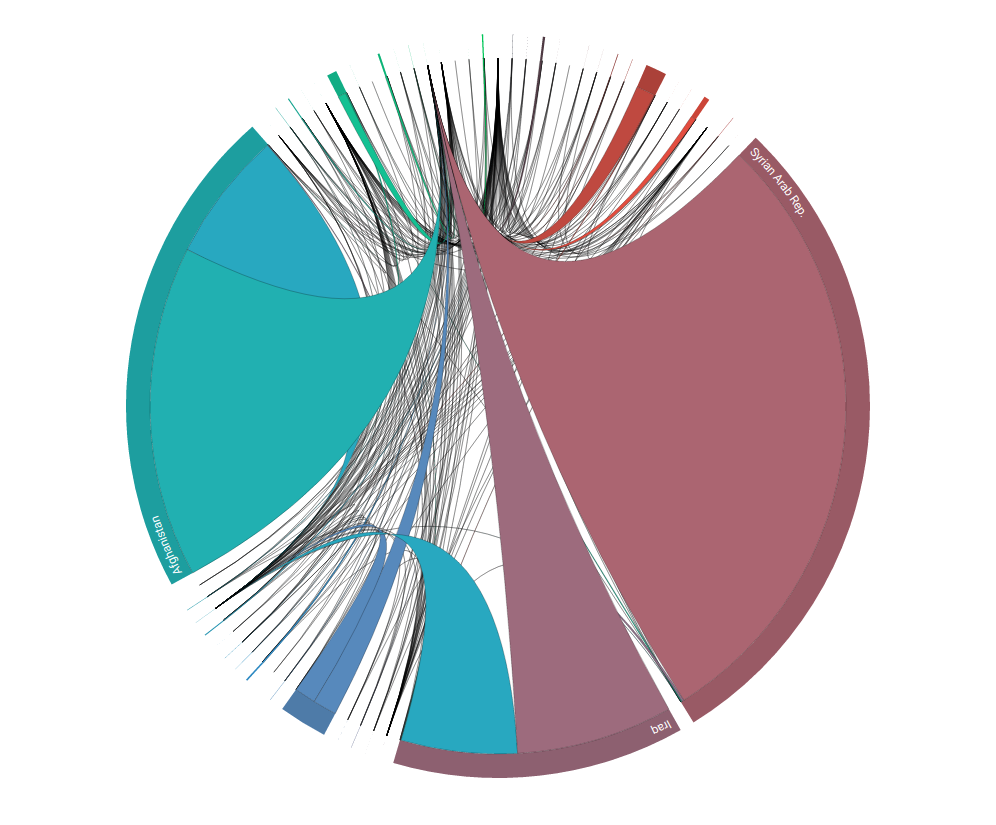
\includegraphics[width=145mm]{img/06_chord_immigration_to_cr_1}
	\caption{D3.js Chord Visualizer: Immigration to Czech Republic}
    \label{fig:chord-immigration-to-cr-1}
\end{figure}

At first glance it might seem that the highest numbers of asylum seekers in Czech Republic come from Syria, Iraq and Afghanistan. This information might be true but it definitely does not stem from this exact visualization. The given figure is static, so it is not apparent, but in a live visualization it is possible to examine actual sources and targets of displayed chords. Having done that, one quickly finds out that those huge chords from Syria, Afghanistan and Iraq are pointing to Turkey and Serbia and Kosovo. So where is the problem?

It is important to realize how the chord diagram works. It displays relationships between nodes. We selected all countries that have at least some (but probably very minimal) traffic of asylum seekers with Czech Republic. The problem is that the traffic in between those other countries is significantly higher and the actual traffic we are interested in (Czech Republic) is almost irrelevant. The chord diagram visualizes that very clearly.

Our visualizer offers some limited tools to deal with this. For example, we can temporarily remove some nodes from the visualization. If we do that with Turkey and Serbia and Kosovo, we suddenly get much better results (Figure \ref{fig:chord-immigration-to-cr-2}.

\begin{figure}
	\centering
	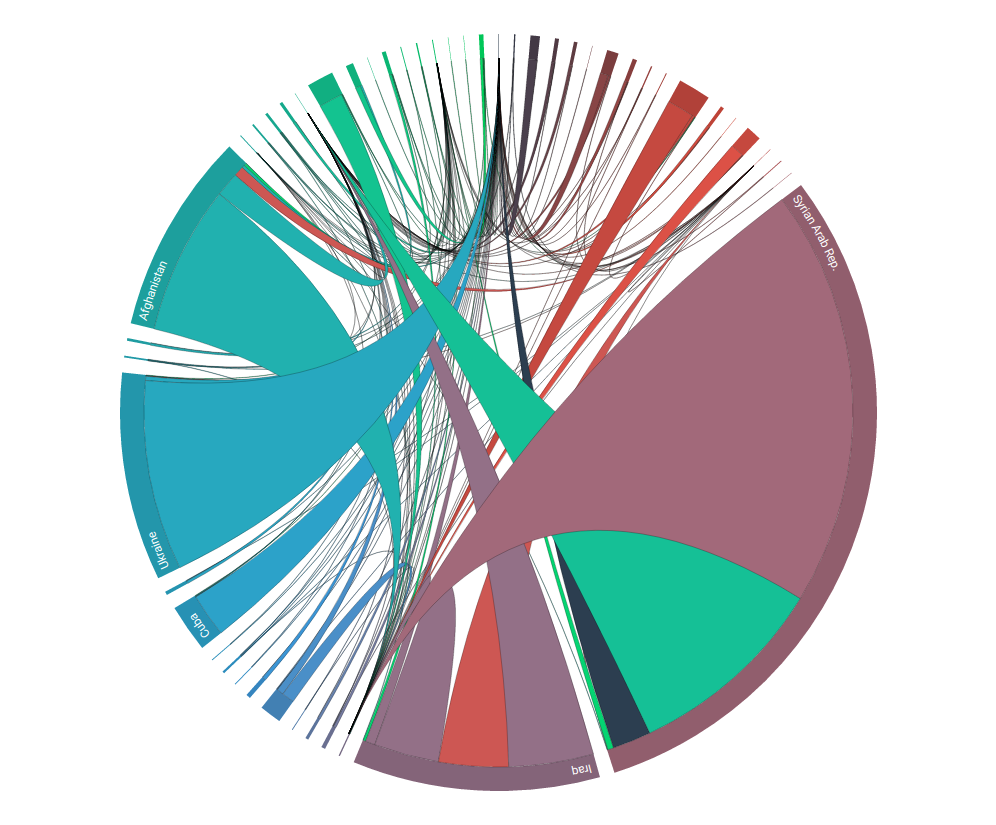
\includegraphics[width=145mm]{img/06_chord_immigration_to_cr_2}
	\caption{D3.js Chord Visualizer: Immigration to Czech Republic without Turkey and Serbia and Kosovo}
    \label{fig:chord-immigration-to-cr-2}
\end{figure}

Even though there is still lots of unrelated and distracting information, we can suddenly see, for example, that there is a large amount of people from Ukraine coming to Czech Republic. The \emph{large amount} in this case is 453 people (compared to the total of 130 000 applications in Turkey).

We solved (or at least diminished) the problem by hiding information. The diagram is supposed to visualize immigration to Czech Republic but there are two countries missing, so it does not correspond to reality. One could say that this diagram actually \emph{lies}. Is this an acceptable way? We believe that this is the strength of our \emph{visualizer} as it allows live interaction with the data. Yes, we temporarily hid some information but we did not remove it . The countries did not disappear from the list. Anyone can always put Turkey and Serbia and Kosovo back in to see the full picture.

One more remark. If you look at Figure \ref{fig:chord-immigration-to-cr-2} again, you still cannot see the node representing Czech Republic. Once again, it is a feature of the chord diagram, not a bug. The relationships here are asymmetrical (the underlying graph is directed). People are coming to Czech Republic, not leaving it. In this visualization, the full circle represents all people seeking asylum from selected countries. There are (almost) no asylum seekers from Czech Republic in this case, so we cannot see Czech Republic. It makes sense but obviously, it is not very practical. For this reason, our \emph{visualizer} offers an option to display asymmetrical chords as symmetrical (i. e., the direction will be ignored). It is a trick, but it gives nice results (Figure \ref{fig:chord-immigration-to-cr-3}).

\begin{figure}
	\centering
	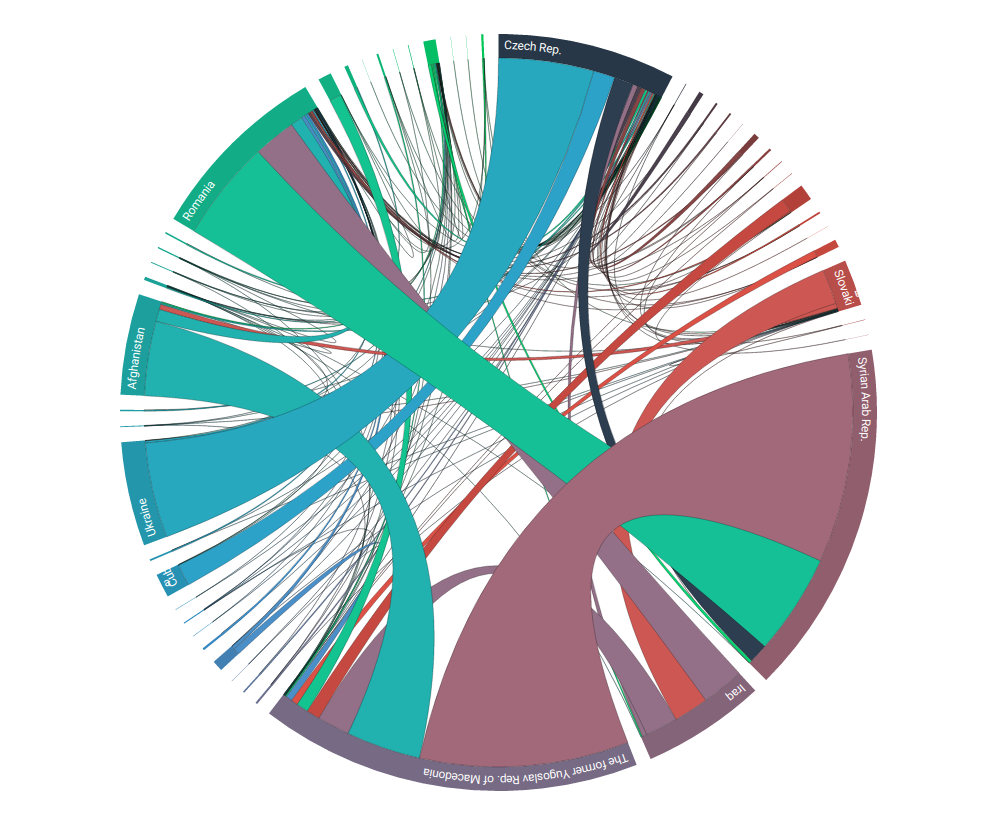
\includegraphics[width=145mm]{img/06_chord_immigration_to_cr_3}
	\caption{D3.js Chord Visualizer: Immigration to Czech Republic without Turkey and Serbia and Kosovo, with enforced symmetrical chords}
    \label{fig:chord-immigration-to-cr-3}
\end{figure}

Besides all the chord related functionality, this \emph{visualizer} also leverages available \emph{platform} and \emph{framework} features, which includes the integration itself but more specifically multiple language support (Subsection \ref{sec:implementation:advanced-features:multiple-language-support}) and custom labels editor (Subsection \ref{sec:implementation:advanced-features:custom-labels-editor}). As you might have noticed on Figure \ref{fig:chord-named-list} with the Visegrad named list, there are countries labeled with Czech names even though the data set itself contains only English variants. The Czech translations have been provided using the custom labels editor. You also could have noticed that the column descriptions in the search dialog (Figure \ref{fig:chord-search-dialog}) are Czech as well. The language variants are included directly in the data set and the \emph{framework} automatically extracts them (Subsection \ref{sec:implementation:advanced-features:label-dereferencering}).

\subsection{Application user interface}

The \emph{application} interface is very similar to the \emph{configurator}. The end user is not allowed to manipulate with the \emph{named lists} (create, delete, search for new nodes) but he can switch between them and toggle individual nodes in lists. 


\begin{figure}
	\centering
	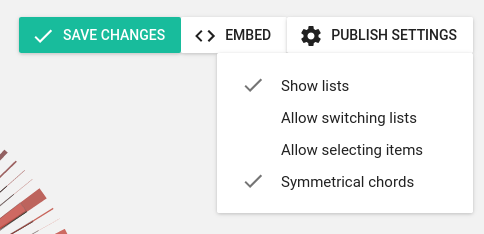
\includegraphics[width=50mm]{img/06_chord_publish_configuration_interface}
	\caption{D3.js Chord Visualizer: Published application interface configuration}
    \label{fig:chord-publish-configuration-interface}
\end{figure}

The \emph{application} interface is to an extent configurable. The application owner can decide to hide the lists, disable list switching or disable node selecting (Figure \ref{fig:chord-publish-configuration-interface}). The idea is still the same. The published application should be tailored to the target audience. For example if necessary, the whole application can be reduced to the chord diagram itself and all interactive elements are either disabled or hidden (Figure \ref{fig:chord-visegrad-published}).

\begin{figure}
	\centering
	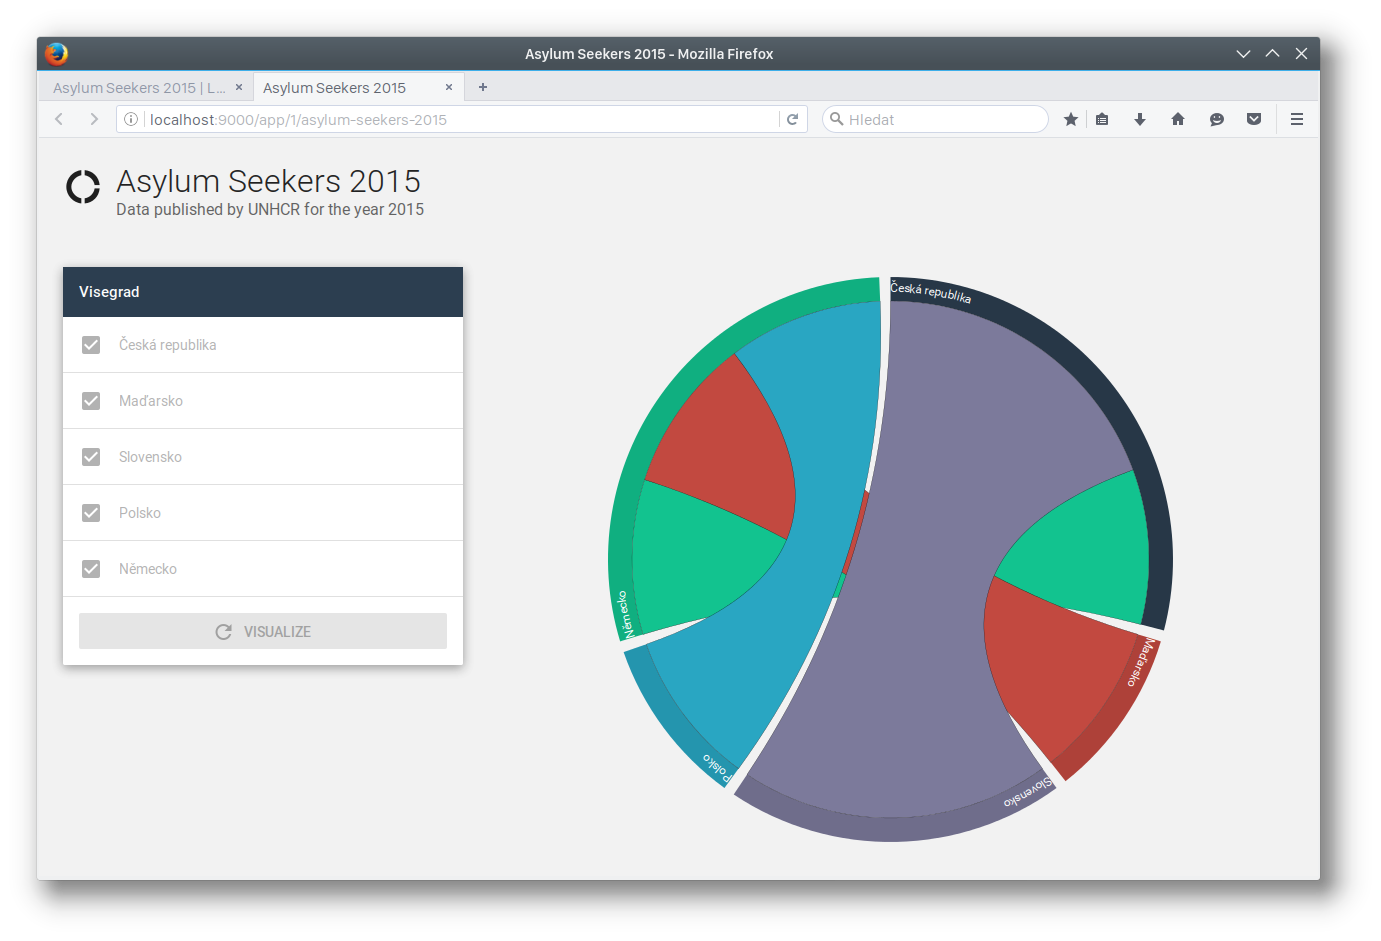
\includegraphics[width=145mm]{img/06_chord_visegrad_published}
	\caption{D3.js Chord Visualizer: Published application which is completely static (regarding interactivity, the data are loaded live) but the user can still see this list of visualized countries. (Note: we are aware that Germany is not a Visegrad member but without Germany there would not be much to visualize.)}
    \label{fig:chord-visegrad-published}
\end{figure}

The chord \emph{visualizer} also offers improved ways of sharing the output via embedding (i. e., inserting the visualizations in external web pages). Each diagram defined by a \emph{named list} can be embedded separately using a unique URL (Figure \ref{fig:chord-embed-configuration}). For example, the user might create several different visualizations based on the same data set and then use all of them in a single article.

\begin{figure}
	\centering
	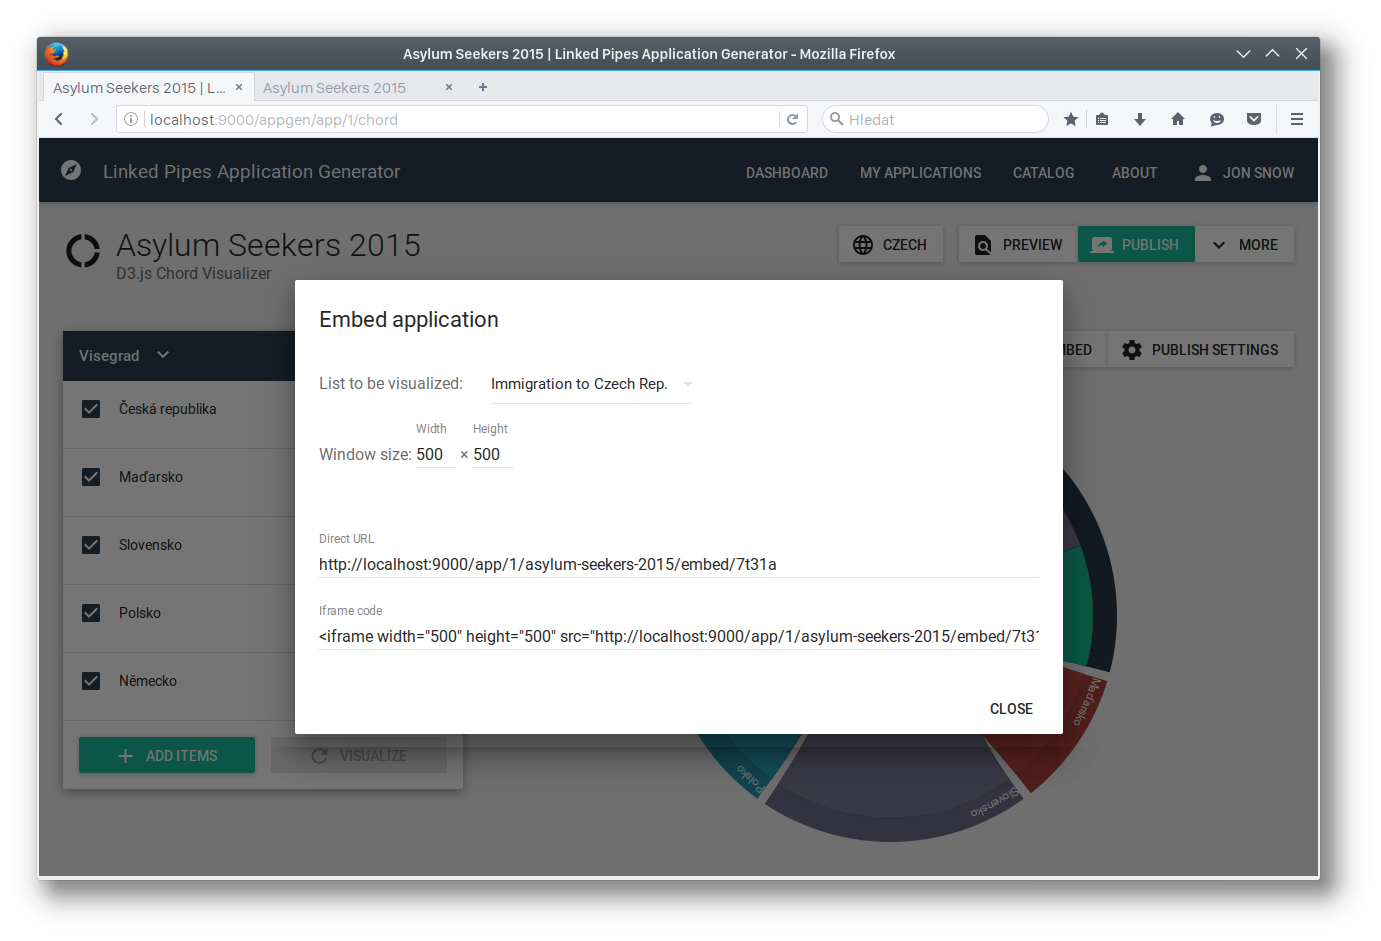
\includegraphics[width=145mm]{img/06_chord_embed_configuration}
	\caption{D3.js Chord Visualizer: Embed application dialog}
    \label{fig:chord-embed-configuration}
\end{figure}

\subsection{Implementation details}

% [cite: https://d3js.org/]
In frontend, the actual chord visualization is powered by the D3.js library. This library was not exactly designed with React in mind and had to be somehow integrated into the application. Besides that, the frontend is simply following concepts that have been described before (Section \ref{sec:implementation:integrating-visualizer}).

% TODO: reformulate 
What we have done in backend was more interesting. We implemented two brand new backend services, \texttt{FresnelService} (responsible for extracting FRESNEL \emph{lenses} and searching the data set) and \texttt{RgmlService} (responsible for loading graph related data from the data set). In the following chapters, we will focus on some of the more interesting problems that we came across when developing these services. Specifically, we will talk about working in general with a graph represented in RDF, about calculating the adjacency matrix for the chord diagram and lastly about implementing the full text search on top of the fresnel vocabulary.

\section{Google Maps Visualizer}
% * <tobiaspotocek@gmail.com> 2016-06-27T13:27:17.697Z:
%
% > Google Maps Visualizer}
%
% Visualizer ještě projde nějakým tím lehkým faceliftingem, tak teprve pak doplním obrázky do kapitoly.
%
% ^.
Google Maps Visualizer focuses on visualizing geospatial information. It shows RDF resources containing GPS coordinates on a map in a form of markers. If the data set supports it, it allows the user to filter the resources.

This \emph{visualizer} was already implemented in LinkedPipes Visualization, so we were able to re-use the LDVM \emph{visualizer component} definition and also all the backend code responsible for extracting RDF data from the \emph{pipeline evaluation}. We only had to implement the frontend part, specifically the \emph{configurator} and \emph{application} interfaces.

For these reasons, this chapter will be rather short and it will not go into technical details. Instead, we will rather focus on the comparison between the original \emph{visualizer}, which is part of LinkedPipes Visualization, and our own implementation that utilizes the capabilities of the \emph{application generator}. 

\subsection{Sample data set}

%[cite: http://internal.opendata.cz/sparql?default-graph-uri=&query=%0D%0Aselect+*+where+%7B%0D%0A%0D%0A%3Chttp%3A%2F%2Flinked.opendata.cz%2Fresource%2Fdataset%2Fmzp.cz%2Fippc%3E++%3Fo+%3Fp+%0D%0A%7D+LIMIT+100&format=text%2Fhtml&timeout=0&debug=on]

We will demonstrate the capabilities of this \emph{visualizer} using only a single data set, \textbf{Registry of business subjects in Czech Republic} [cite and use the real name]. As the name suggests, this data set contains business subjects. Each business subject has GPS coordinates of its residence. These entities will be visualized on the map.

Each business subject is put into two categories. The \emph{primary category} and the \emph{secondary category}. The data set contains list of available categories. The user will be allowed to filter the business subjects using these categories.

\subsection{Filtering}

Filtering is an essential part of this \emph{visualizer}. It works similarly to what the reader might be used to for example from browsing products in e-shops. Just for now, let us say that the data set does not contain geospatial entities but rather laptops. A laptop has properties like brand, screen size or operating system. Each of these properties defines a \emph{filter} (e.g. brand) with a list of available \emph{values} (e.g. Asus, Dell, Apple etc). The user can select an arbitrary number of \emph{values} for each \emph{filter} to create filtering criteria. For a laptop to be included in the result set, it has to match all the criteria (conjunction). For a laptop to match a criterion, its property \emph{value} corresponding to the criterion \emph{filter} must be one of the \emph{values} selected by the user (disjunction). For example, by selecting Asus and Dell as the brand, 15 inches as the screen size and Windows 10 as the operating system, the user will get all 15-inch laptops with Windows 10 manufactured either by Asus or Dell.

If the user selects all \emph{values} for a \emph{filter}, it is just as if the \emph{filter} was not there at all. It has no impact on the result set. On the other hand, if the user selects no \emph{values} for a \emph{filter}, the results set is always empty (no laptops can meet the criteria).

Available \emph{filters} and their \emph{values} has to be explicitly defined in the data set. In our sample data set, as already mentioned, those are the \emph{primary category} and \emph{secondary category}.

\subsection{Configurator and application user interface}

\emph{Configurator} and \emph{application} interfaces are very similar. Both of them feature a map and a sidebar on the left with \emph{filters}. The key difference is that in the \emph{configurator} interface, the \emph{filters} can be displayed in two modes: configuration and preview. The \emph{application} interface shows the \emph{filters} always in the same way which corresponds to the preview mode.

The idea is that by configuring the \emph{filters} the user can significantly affect the shape of the published application. Here are some examples.

\begin{itemize}
\item A \emph{filter} can be \textbf{disabled}. A disabled \emph{filter} is interpreted as if all its \emph{values} have been selected, i.e., it has no impact on the selected output. This filter is completely hidden in the published application.
\item A \emph{value} can be \textbf{enforce}. That means that it is always selected.
\item A \emph{value} can be \textbf{disabled}. That means that it cannot be selected. This \emph{value} is completely hidden in the published application.
\item A \emph{filter} can be switched between \textbf{checkbox} mode and \textbf{radio} mode. In checkbox mode, an arbitrary number of \emph{filter} \emph{values} can be selected. In radio mode, only one \emph{value} can be selected. The mode names correspond to the appropriate form controls.

\end{itemize}
Thanks to the enforcing and disabling of certain \emph{values}, it is possible to create default filters that are always applied. That essentially means that the published application can be based just on a subset of the input data. If we go back to our example with laptops, one could generate a browser of Dell laptops filterable by screen size. To achieve that, one would have to disable the operating system \emph{filter}, enforce the Dell \emph{value} and disable all other \emph{values} for the brand \emph{filter}.

By either fixing or disabling all \emph{filters} and \emph{values}, it is actually possible to generate a completely static application which might also make sense in certain situations. Moreover, It is possible to disable the sidebar with \emph{filters} completely which reduces the published application just to a static map with pre-selected markers.

Besides the filter configuration, the \emph{configurator} interface also allows the user to fix the default map position and zoom level. Naturally, it also implements the available universal features, like multi language support and custom labels editor (e.g. it is possible to rename \emph{filters}  and their \emph{values}).

% TODO: marker infowindows/tooltips

\subsection{Advantages over LinkedPipes Visualization}

The reader might be wondering why we presented a sample data set but then we used a completely different example to explain how the filtering works. The reason is that the presented data set is if not actually broken then at least very confusing (its quality is a little poor). That does not make it very suitable for explaining principles, but it makes it perfect for demonstrating the abilities of our \emph{visualizer}.

As explained, each business subject has a \emph{primary category} and a \emph{secondary category}. Those are two properties that would both make up one \emph{filter} each. Since the data is in RDF, each property is actually an RDF resource with a unique URI. The problem here is that they both have the same label and they both contain exactly the same \emph{values} which means that they will both look exactly the same to the user. The label can be approximately translated as \textit{"Businesses as defined by the 1st attachment of the integrated prevention law"}.

If we go back to the example of the e-shop selling laptops, there is one big assumption: We assume that the user is at least to some extent familiar with the nature of the product. E.g. he knows what the brand or the screen size is. Therefore we assume that he would intuitively understand what happens if he selects in the filters the brand Dell and the screen size 15 inches. In case of our data set, however, not only might the user have no idea what \textit{"Businesses as defined by the 1st attachment of the integrated prevention law"} are in the first place, but also the fact that this property is there twice would confuse him even more. 

It is important to say that this is exactly what the LinkedPipes Visualization visualizer would show. Two identical \emph{filters} with confusing names and identical \emph{values}. We can hardly expect any intuition from the user here. Plus the list of \emph{values} is fairly long and because of the way it is displayed, the user might not realize that there are actually two \emph{filters}. That might cause another problem: if the user is not aware of the second \emph{filter} and selects no \emph{values} for it, he will always get an empty result set.

Interestingly enough, the current implementation in LinkedPipes Visualization does not suffer from this problem but only by a sheer coincidence. Firstly, even though each business subject is put into two categories (\emph{primary} and \emph{secondary}), they are always the two same categories, i.e., both the \emph{primary} and the \emph{secondary category} points to the same RDF resource with the same URI. Secondly, there is a bug in the  user interface implementation of filters in LinkedPipes Visualization causing that if the user selects a \emph{value} in the \emph{primary category} \emph{filter}, this \emph{value} (identified by a URI) gets also automatically selected in the \emph{secondary category} \emph{filter}.

In the example with laptops this would mean that each laptops would have two brands which would however be always the same (e.g. a laptop would have the "primary" brand Dell and also the "secondary" brand Dell). To filter Dell laptops, we would need to specifically select Dell in both brand \emph{filters}. Because of the UI bug, this would be done automatically for us.

The reader might object that this behavior in the UI is not a bug but is rather intentional as it follows the structure of the data. Let us imagine that a laptop has two new properties. A chassis color and a keyboard color. They would correspond to two new \emph{filters} with exactly the same \emph{values} (a list of several predefined colors). Clearly, we want to select the colors independently. Selecting red for the chassis should not automatically mean selecting red for the keyboard. Note that structure of this example is identical to our data set. The only difference is that our \emph{primary category} and \emph{secondary category} both have the same label, so they appear as identical. But they are not. Their URIs are different and that is what matters.

To sum it up: a visualization of this data set generated with LinkedPipes Visualization would expose all these flaws to any end user that would come across this visualization. This makes the visualization not very user friendly. On the other hand, in our \emph{application generator} we can utilize the configuration phase to fix these issues and deliver much better user experience (not to mention that our implementation does not suffer from the aforementioned bug). Specifically, we could undergo the following steps:

\begin{itemize}
\item \textbf{Rename the \emph{filters}.} Using the custom labels editor we could provide better and more explanatory names to the \emph{filters} so that the user would get a better idea of their behavior. Just using "Primary category" and "Secondary category" as names would probably improve the overall experience. The original name, \textit{"Businesses as defined by the 1st attachment of the integrated prevention law"}, rather just explains what the \emph{values} are and this information could go to the application description.
\item \textbf{Disable one of the \emph{filters}.} As in this data set both categories are always the same, disabling one of the filters will not cause the visualization to lose any information or functionality and it will only improve the experience.
\item \textbf{Reduce the data set}. Even if one of the \emph{filters} is disabled, there is still more than 60 \emph{values} to choose from. Perhaps we could instead of one big application generate multiple smaller applications where each would utilize default filters to visualize only a specific subset of the data set.
\end{itemize}

Using our \emph{application generator}, we were able to take a data set of poor quality and turn it into a useful and user-friendly application. Which is something that would not be possible with LinkedPipes Visualization.

One last remark. The \emph{configurator interface} does not shield the user from these data set related problems. The main advantage is that only the user that generates the application needs to deal with these issues. Once the application is properly generated, it is ready to be comfortably consumed by a way broader audience. In LinkedPipes Visualization, on the other hand, everybody gets the raw visualization and has to make his own sense out of the data.
